\graphicspath{{05-EMR/Figures/}}

\section{Electron Muon Ranger}
\label{Sect:EMR}

\subsection{Introduction}
\label{SubSect:EMR_Intro}

The Electron-Muon Ranger (EMR) is a fully-active scintillator detector~\cite{2016JInst..11T10007}. It can be classified as a tracking-calorimeter as its granularity allows for track reconstruction. The EMR consists of extruded triangular scintillator bars arranged in planes. One plane contains 59 bars and covers an area of 1.27\,m$^2$. Each even bar is rotated by 180 degrees with respect to the odd one. A cross-section of bars and their arrangement in a plane is shown in Fig.~\ref{fig:EMR}. This configuration does not leave dead area in the detector for particles crossing a plane with angles that do not exceed 45 degrees with respect to the beam axis. Each plane is rotated through 90 degrees with respect to the previous one, such that a pair of planes defines a horizontal and vertical $(x, y)$ interaction coordinate. The light, produced when a particle crosses a bar, is collected by a wave-length shifting (WLS) fibre glued inside the bar. At both ends, the WLS fibre is coupled to clear fibres that transport the light to a photomultiplier tube (PMT). Signals produced in a plane are read out collectively on one end by a single-anode PMT for an integrated charge measurement and separately on the other by a multi-anode PMTs for individual bar hit reconstruction. The full detector is composed of 24 X--Y modules for a total active volume of $\sim 1$\,m$^3$.

\begin{figure}[htb!]
	\begin{center}
		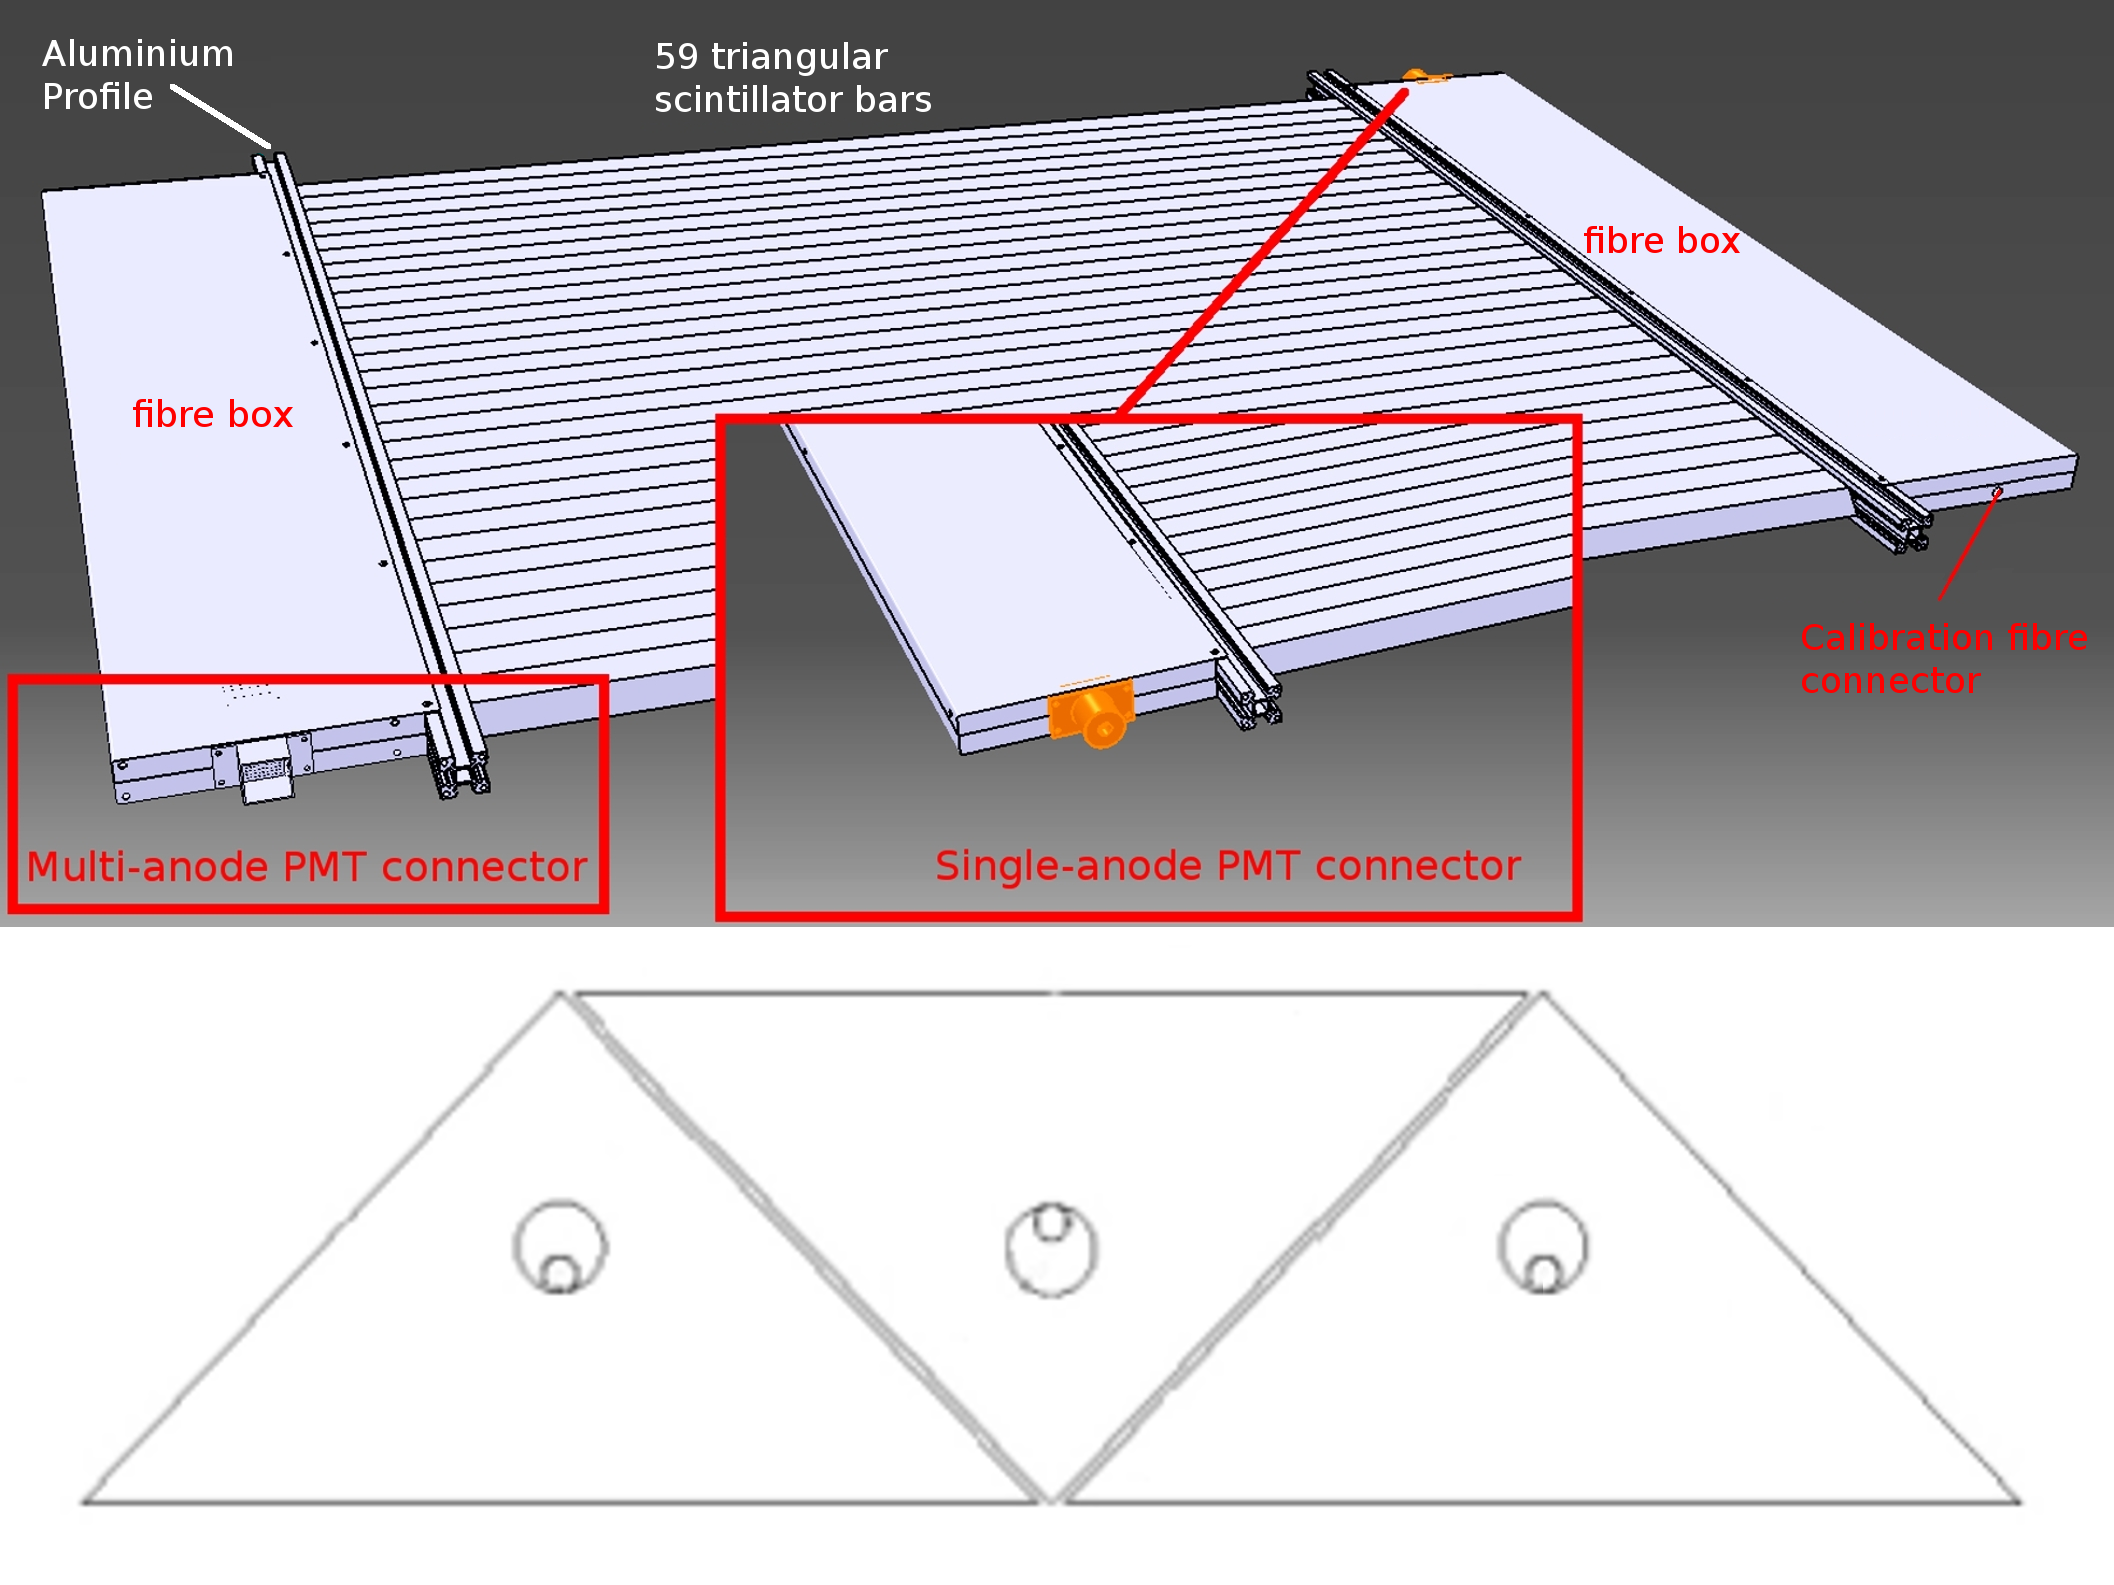
\includegraphics[width=0.465\columnwidth]{EMR1.png}
		\hfill
		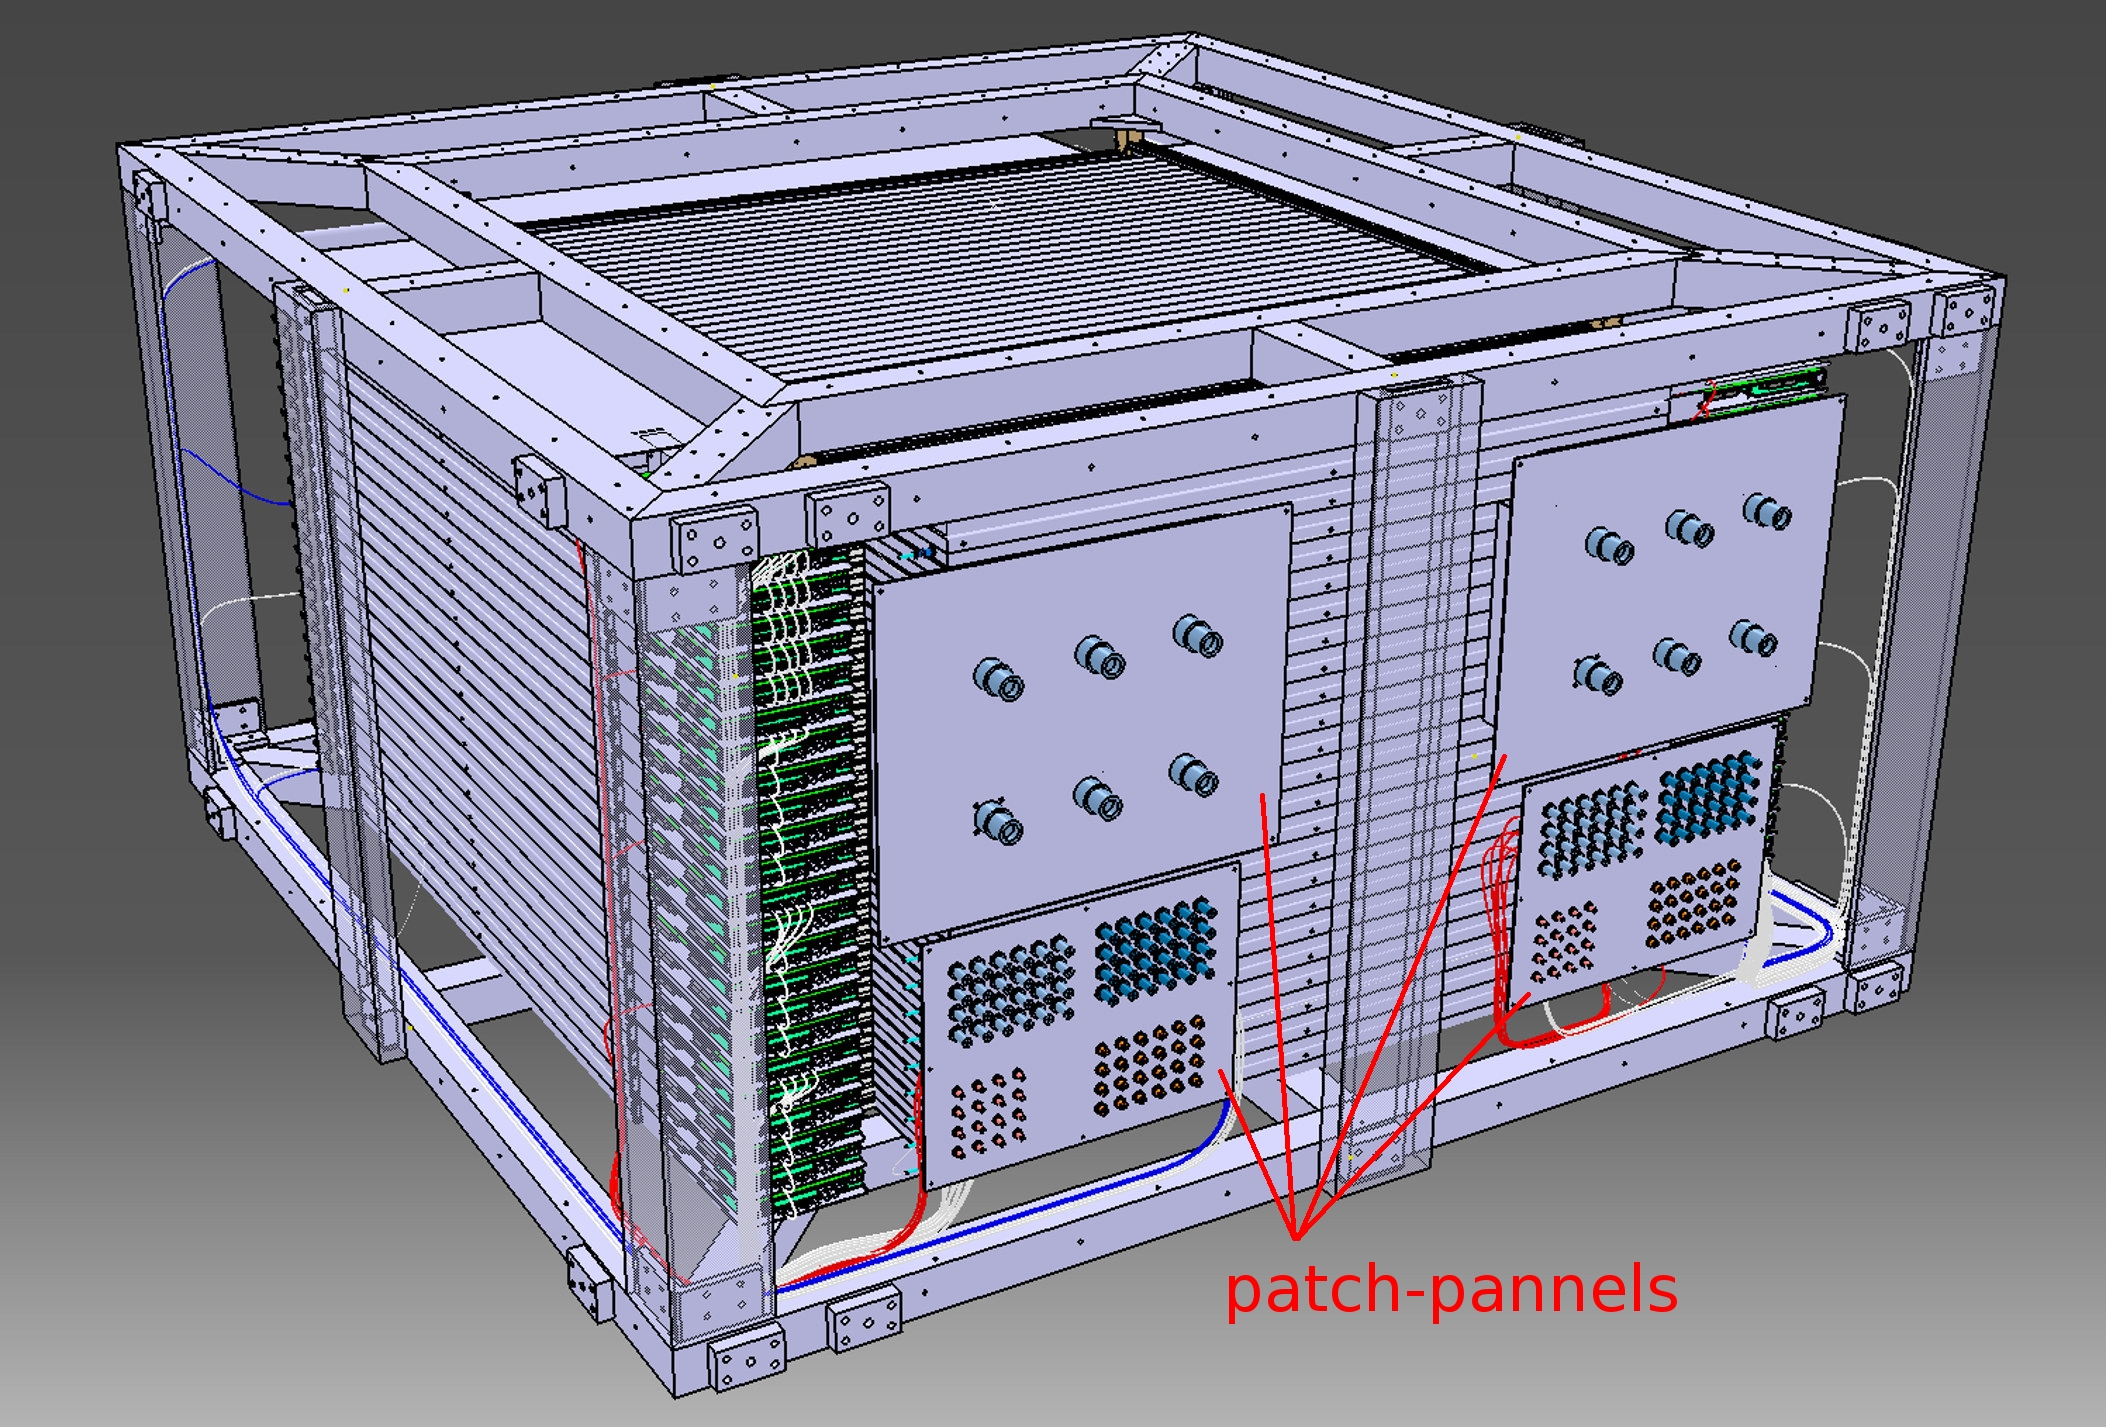
\includegraphics[width=0.515\columnwidth]{EMR2.jpg}
		\caption{Drawing of one EMR plane (top left), cross section of 3 bars and their wavelength shifting fibres (bottom left) and drawing of the full detector and its supporting structure (right).}
		\label{fig:EMR}
	\end{center}
\end{figure}

An array of analyses were conducted to characterize the hardware of the EMR and determine whether the detector performs to specifications~\cite{Drielsma:2017doj}. The clear fibres coming from the bars were shown to transmit the desired amount of light, and only four dead channels were identified in the electronics. The level of crosstalk is within acceptable values for the type of multi-anode photomultiplier used with an average of $0.20\pm0.03$\,\% probability of occurrence in adjacent channels and a mean amplitude equivalent to $4.5\pm0.1$\,\% of the primary signal intensity. The efficiency of the signal acquisition, defined as the probability of recording a signal in a plane when a particle goes through it in beam conditions, reached $99.73\pm0.02$\,\%.

The primary purpose of the EMR is to distinguish between muons and their decay products, identifying
muons that have crossed the entire cooling channel. Muons and electrons exhibit distinct behaviours in the detector. A muon follows a single straight track before either stopping or exiting the scintillating volume, while electrons shower in the lead of the KL and create a broad cascade of secondary particles. Two main geometric variables, the plane density and the shower spread, are used to differentiate them. The detector is capable of identifying electrons with an efficiency of 98.6\,\%, providing a purity for the MICE beam that exceeds 99.8\,\%. The EMR also proved to be a powerful tool for the reconstruction of muon momenta in the range 100--280\,MeV/$c$~\cite{2015JInst..10P2012A}.

\subsection{Performance}
\label{SubSect:EMR_Performance}

The performance of the EMR detector is assessed at three levels of resolution with the data acquired during the 2017/02 and 2017/03 ISIS user cycles. The performance of the hardware itself is evaluated by analysing the characteristics of raw photomultiplier signals. The reconstruction efficiency is assessed by looking at higher level quantities. The performance of the detector as an electron tagging device is measured.

\subsubsection{Hardware efficiencies}
The data sets used to evaluate the detector hardware efficiencies are summarized in Table~\ref{tab:emr_eff_data_sets}. The MICE beam line is tuned to the highest attainable momentum to maximize the transmission to the EMR detector and increase the range of particles in the detector. In this configuration, the beam line produces pions and muons in comparable quantities, along with positrons. The particle species are identified by evaluating their time-of-flight between TOF1 and TOF2.
%The time-of-flight distribution for muons, pions and positrons is represented in figure~\ref{fig:emr_eff_tof}. The muons and pions peaks are fitted with a sum of two Gaussians of the form
%\begin{equation}
%f_{\mu,\pi}(t_{12}) = \frac{A_{\mu,\pi}}{\sqrt{2\pi}\sigma_{\mu,\pi}} \exp\left[-\frac{(t_{12}-t_{\mu,\pi})^2}{2\sigma_{\mu,\pi}^2}\right].
%\end{equation}
Only the particles with a time-of-flight between 28 and 28.75\,ns, i.e. compatible with the muon hypothesis, are included in the analysis sample.

\begin{table}[htb!]
	\centering
	\begin{tabular}{c|c|c|c|c|c|c}
		Run ID & Date & Type & Momentum & Spills & Triggers & EMR events \\
		\hline
		9619 & 19/09/2017 & $\pi^+$ & 400 MeV/$c$ & 2289 & 265312 & 36775 \\
		9620 & 19/09/2017 & $\pi^+$ & 400 MeV/$c$ & 5388 & 668026 & 107578 \\
		\hline
		\multicolumn{3}{c}{} & \textbf{Total} & 7677 & 933338 & 144353
	\end{tabular}
	\caption{Summary of the data sets used to measure the efficiency of the EMR in the 2017/02 ISIS user cycle.}
	\label{tab:emr_eff_data_sets}
\end{table}

%\begin{figure}[htb!]
%    \begin{center}
%    	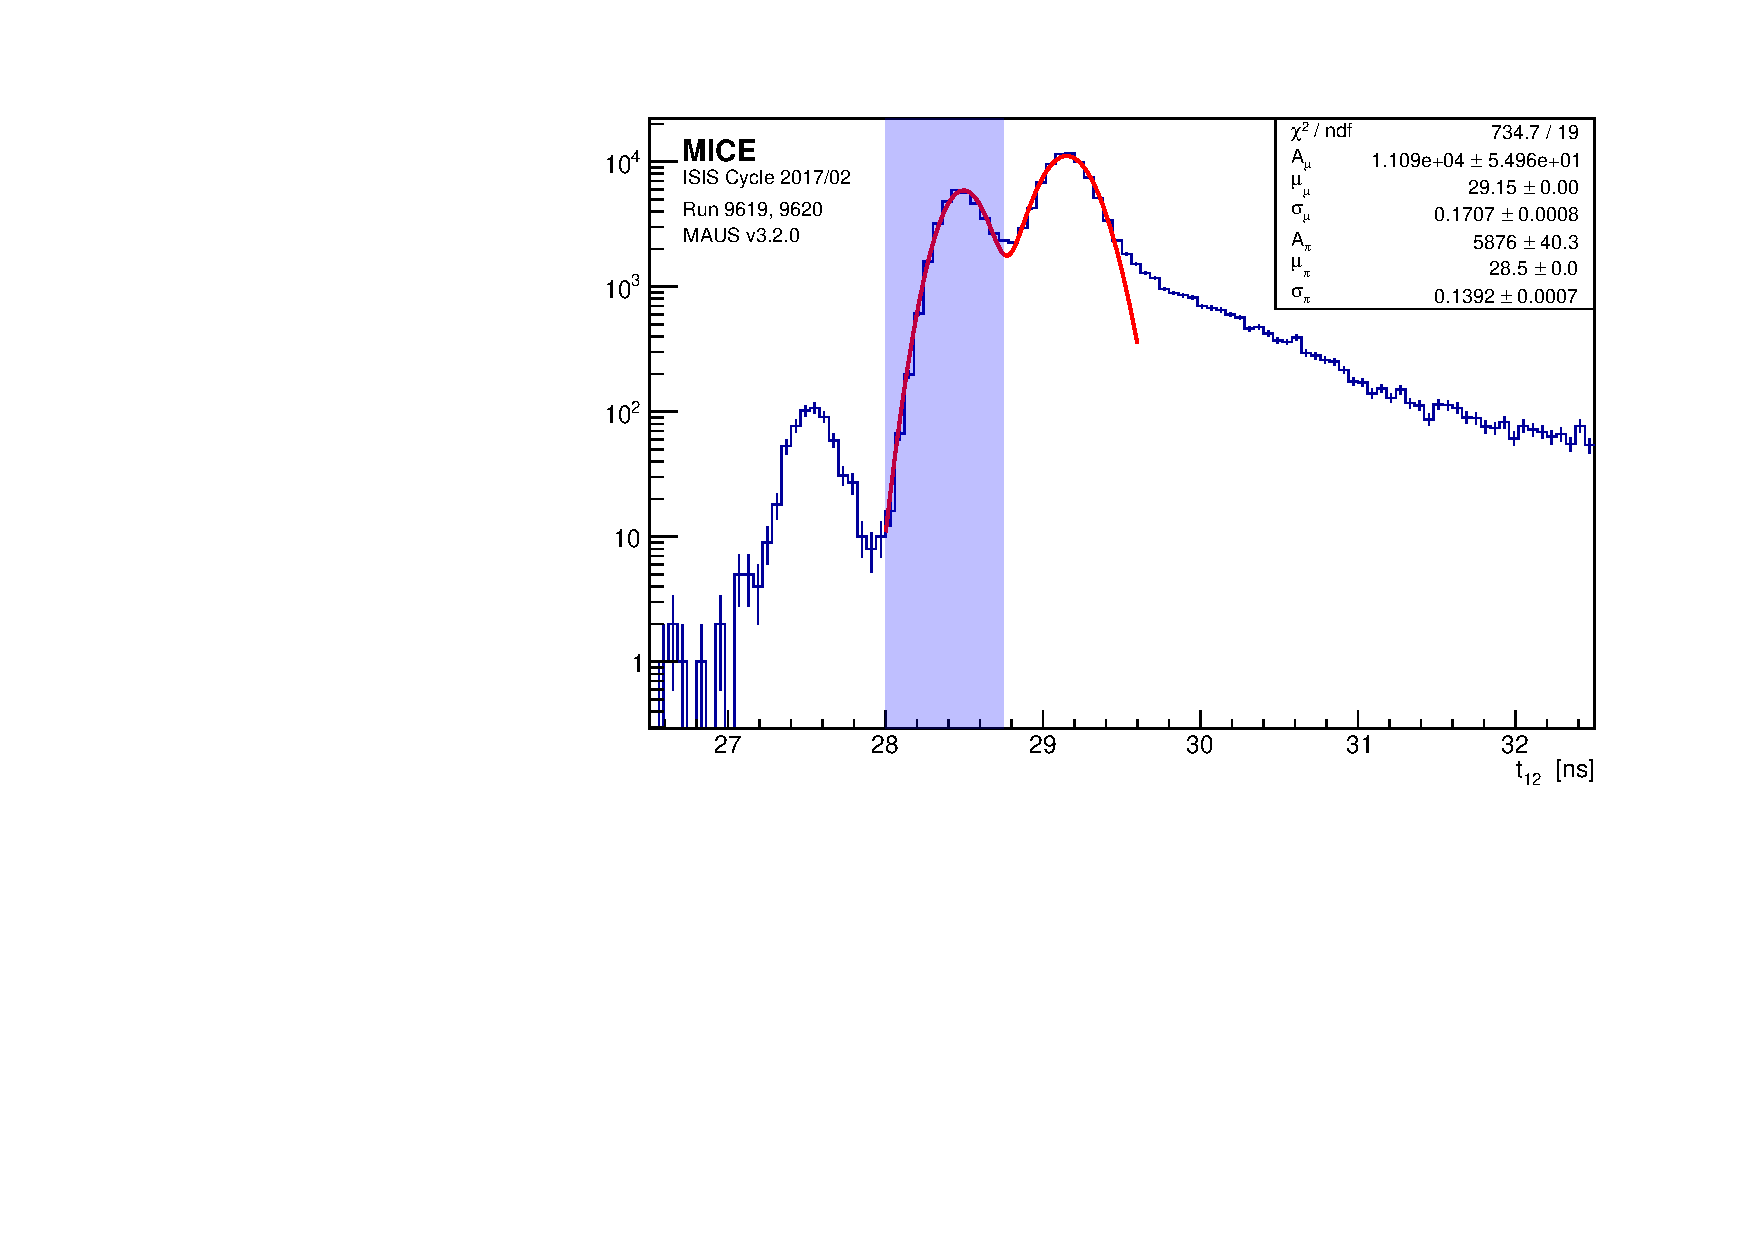
\includegraphics[width=0.7\columnwidth]{tof12.pdf}  		
%    	\caption{Time-of-flight of positrons, muons and pions for the 400\,MeV/$c$ pionic beam line used in the EMR efficiency analysis. The blue band represents the selected %range.}
%    	\label{fig:emr_eff_tof}
%    \end{center}
%\end{figure}

A muon that makes it into the analysis sample has a momentum larger than 350\,MeV/$c$ right before TOF2. It is expected to cross both TOF2 and the KL without stopping and penetrate the EMR. In practice, the probability of creating an EMR event, i.e. to produce hits in the detector is $99.62\pm0.03\,\%$. The minor inefficiency may be attributed to pions in the muon sample that experience hadronic interactions in the KL. If hits are produced in the detector, space points are reconstructed $98.56\pm0.06\,\%$. This inefficiency may be associated with muon that decay between TOF2 and the EMR and produce scarce hits in the detector.

To evaluate the efficiency of the scintillator planes and their readouts, only the muons which penetrate the entire detector are taken into account. If a signal is recorded in the most downstream plane, it is expected that at least a bar will be hit in each plane on its path and that a signal will be recorded in the single anode PMT.
In $3.26\pm0.02\,\%$ of cases, on average, a plane traversed by a muon will be not produce a signal in its MAPMT and that the most probable amount of bars hit is one, while
a track is missed by an SAPMT $1.88\pm0.01\,\%$ of the time. 

%Figure~\ref{fig:emr_plane_eff} shows the probability of recording a signal in individual MAPMTs and the SAPMTs for each of the 48 planes, given a muon that crosses the whole detector. The most inefficient PMTs miss the track $\sim10\,\%$ of the time.
%
%\begin{figure}[htb!]
%	\begin{center}
%		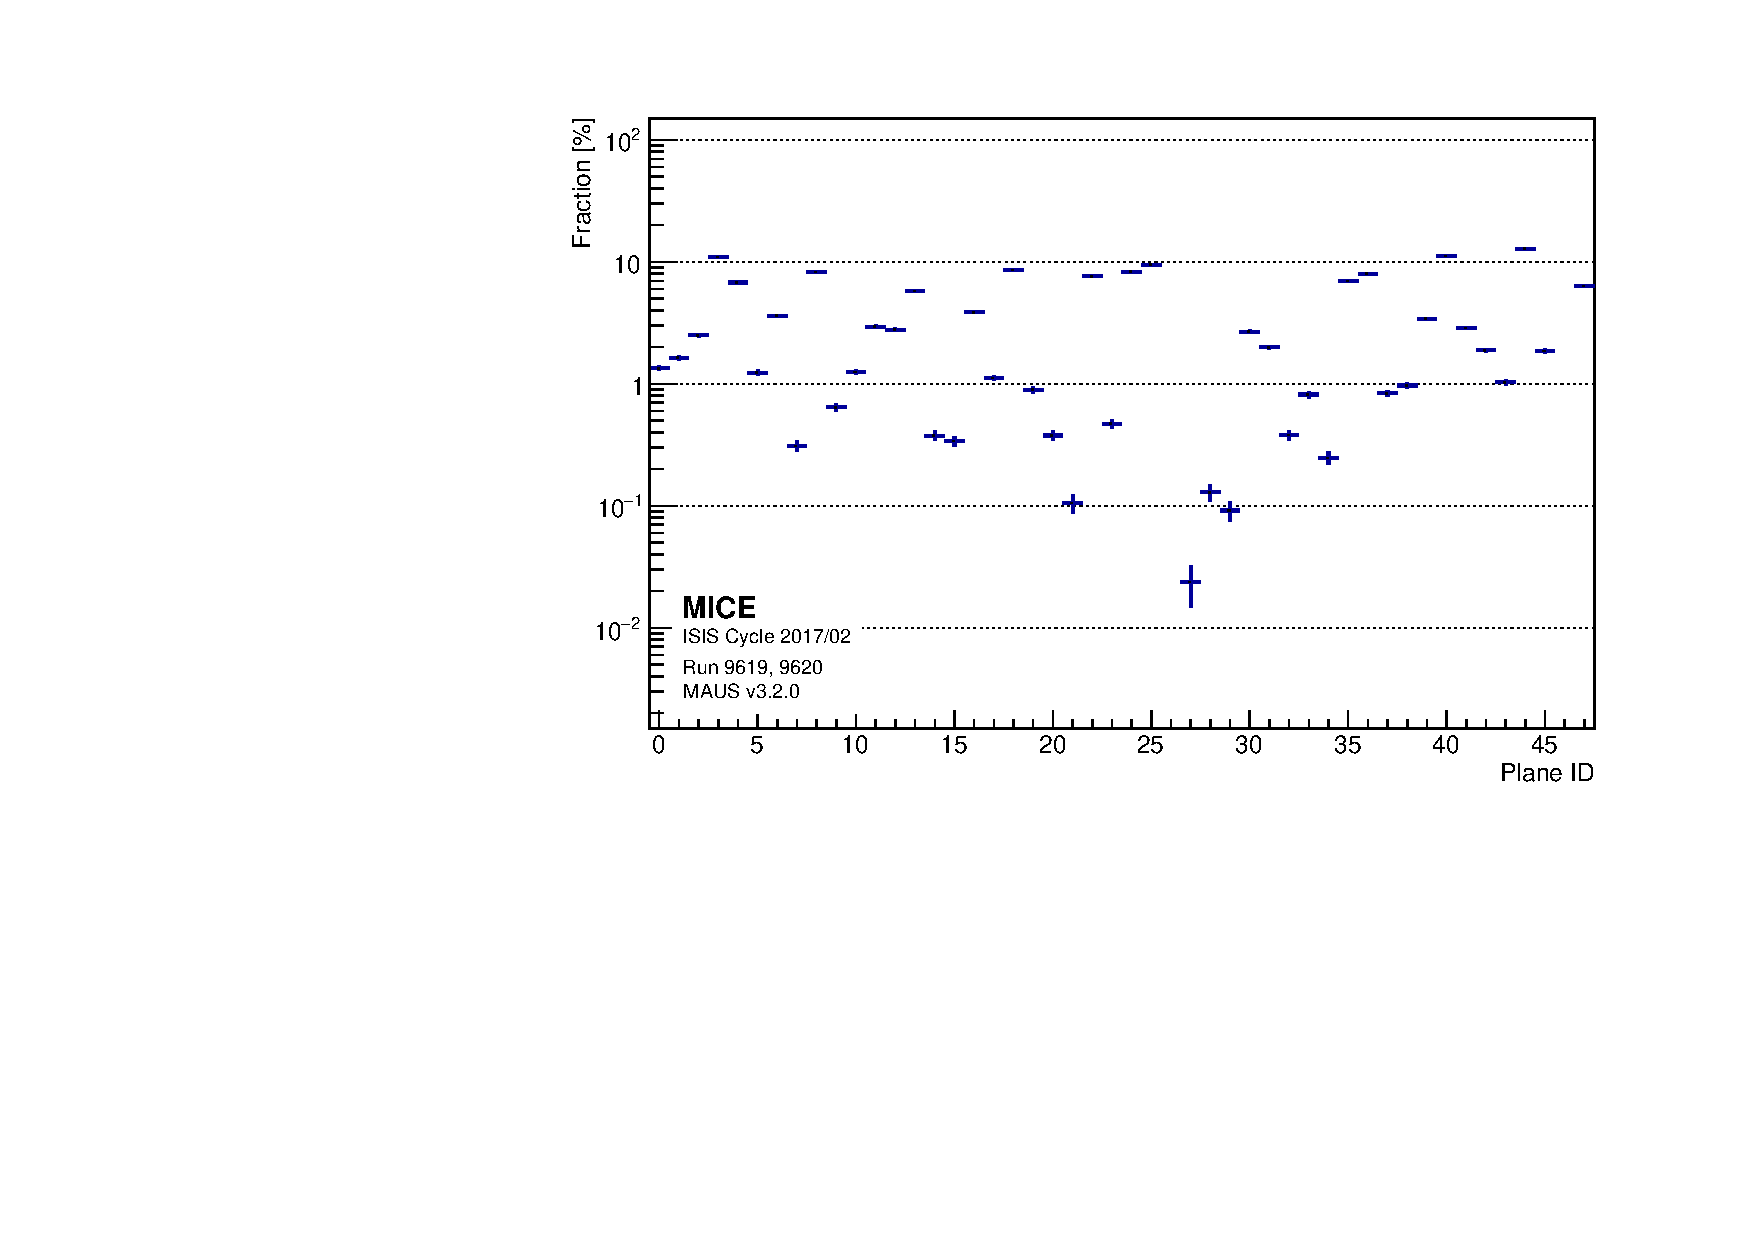
\includegraphics[width=0.49\columnwidth]{missed_mapmt.pdf}
%		\hfill
%		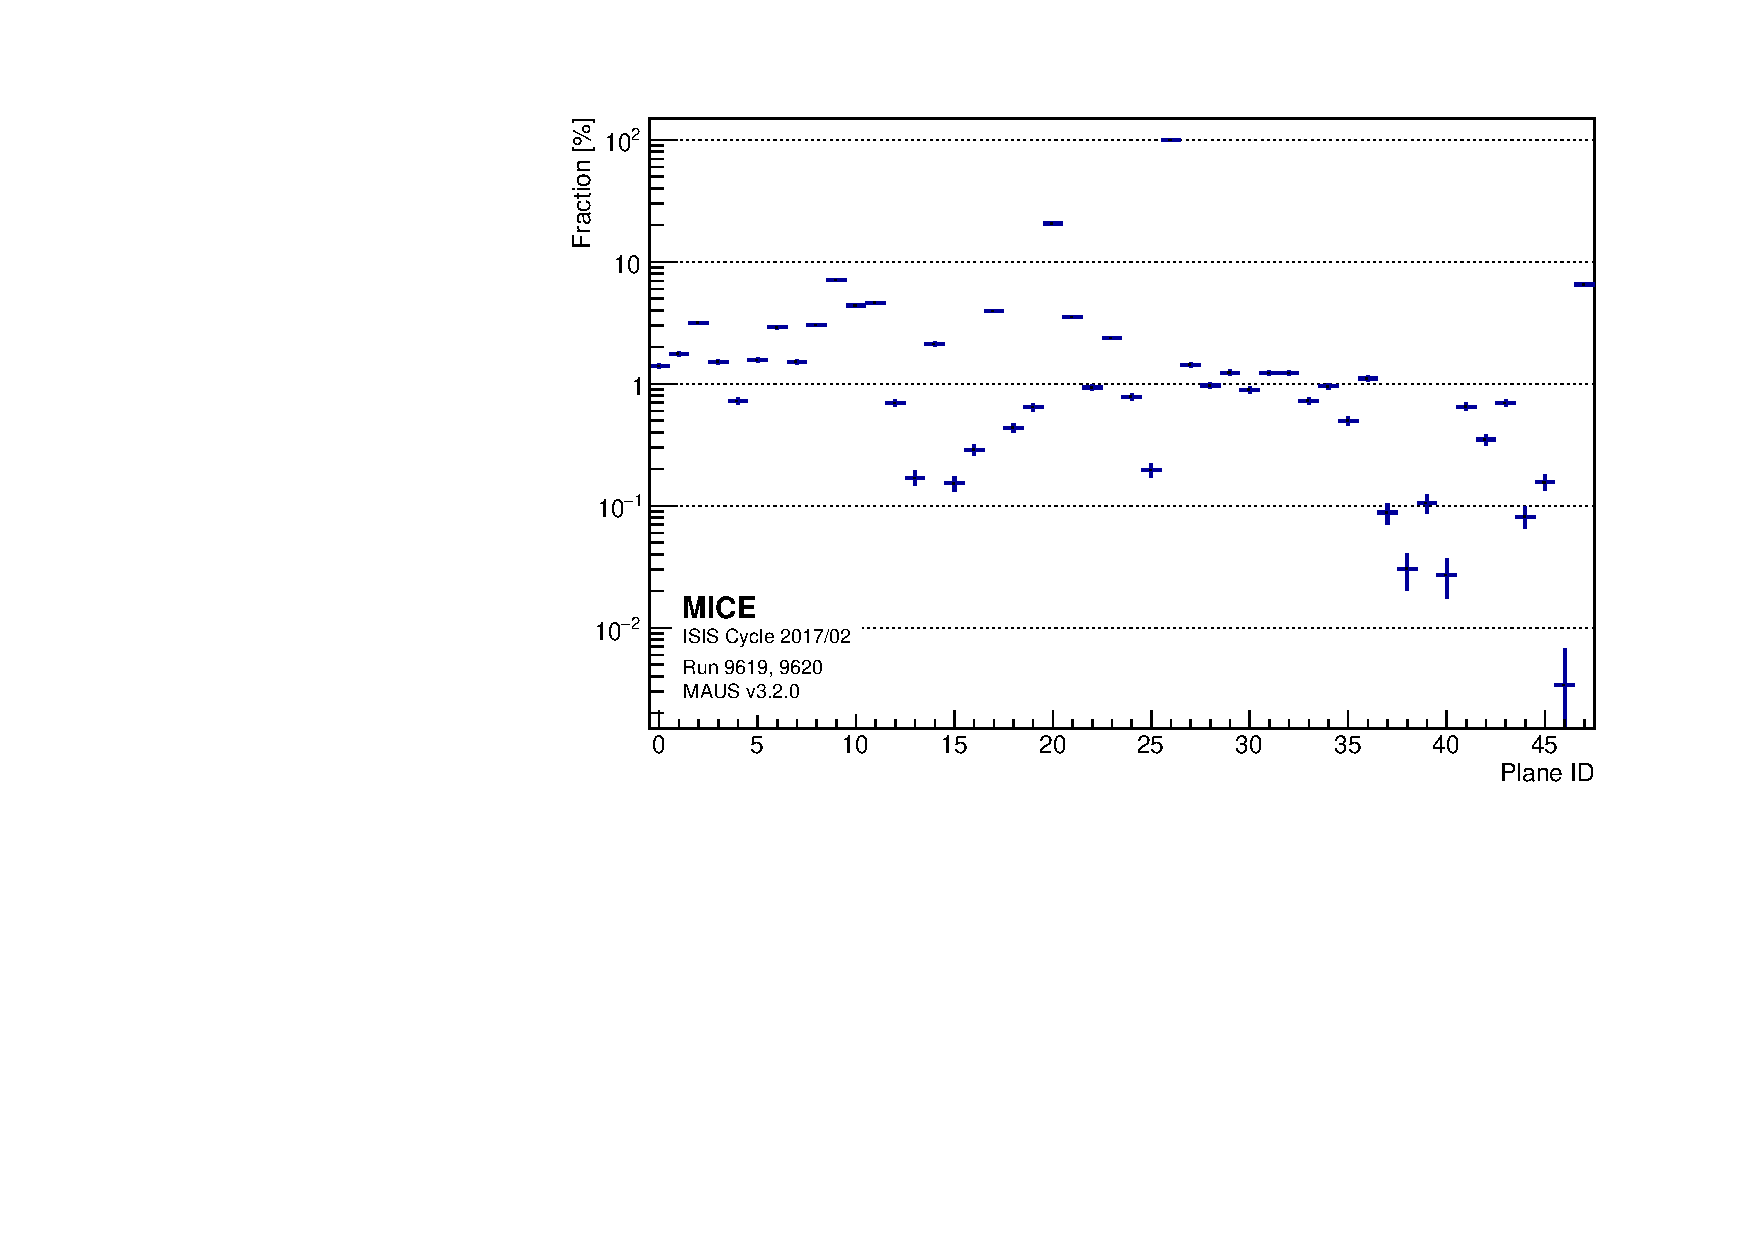
\includegraphics[width=0.49\columnwidth]{missed_sapmt.pdf}
%		\caption{Probability of not producing a single bar hit in the MAPMT (left) and a zero charge in the SAPMT (right) in the 48 individual EMR planes.}
%		\label{fig:emr_plane_eff}
%	\end{center}
%\end{figure}

\subsubsection{Electron rejection}
The main purpose of the Electron-Muon Ranger is to tag and reject the muons that have decayed in flight inside the experimental apparatus. A broad range of beam line momentum settings, summarized in Table~\ref{tab:emr_analysis_data_sets}, is used to characterize its muon selection efficiency. The particle species are characterized upstream of the detector by using the time-of-flight between TOF1 and TOF2 as shown before.
The limits of the peaks are fitted to each setting in order to separate the muons and positrons into two templates upstream of the EMR. Particles that fall above the upper limit of the muon peak are either pions or slow muons and are rejected from this analysis.

\begin{table}[htb!]
	\centering
	\begin{tabular}{c|c|c|c|c|c|c}
		Run ID & Date & Type & Momentum & Spills & Triggers & EMR events \\
		\hline
%		10243 & 24/11/2017 & $\pi^+$ & 140 MeV/$c$ & 4316 & 264642 & ? \\
%		10248 & 24/11/2017 & $\pi^+$ & 140 MeV/$c$ & 4332 & 317583 & ? \\
%		10253 & 25/11/2017 & $\pi^+$ & 140 MeV/$c$ & 285 & 21533 & ? \\
%		10254 & 25/11/2017 & $\pi^+$ & 140 MeV/$c$ & 3852 & 282162 & ? \\
%		10255 & 25/11/2017 & $\pi^+$ & 140 MeV/$c$ & 1409 & 100121 & ? \\
%		10256 & 25/11/2017 & $\pi^+$ & 140 MeV/$c$ & 1660 & 121131 & ? \\
%		\hline
		10268 & 26/11/2017 & $\pi^+$ & 170 MeV/$c$ & 4418 & 328948 & 97452 \\
		10269 & 26/11/2017 & $\pi^+$ & 170 MeV/$c$ & 3695 & 278330 & 82098 \\
		\hline
		10262 & 25/11/2017 & $\pi^+$ & 200 MeV/$c$ & 846 & 28103 & 8769 \\
		10266 & 25/11/2017 & $\pi^+$ & 200 MeV/$c$ & 4365 & 148990 & 45448 \\
		10267 & 26/11/2017 & $\pi^+$ & 200 MeV/$c$ & 4296 & 194207 & 53469 \\
		10275 & 26/11/2017 & $\pi^+$ & 200 MeV/$c$ & 3547 & 126597 & 39114 \\
		\hline
		10261 & 25/11/2017 & $\pi^+$ & 240 MeV/$c$ & 4388 & 228337 & 66335 \\
		10264 & 25/11/2017 & $\pi^+$ & 240 MeV/$c$ & 755 & 32322 & 10041 \\
		10265 & 25/11/2017 & $\pi^+$ & 240 MeV/$c$ & 3336 & 134953 & 43129 \\
		10270 & 26/11/2017 & $\pi^+$ & 240 MeV/$c$ & 222 & 17584 & 4030 \\
		10271 & 26/11/2017 & $\pi^+$ & 240 MeV/$c$ & 66 & 5063 & 287 \\
		10272 & 26/11/2017 & $\pi^+$ & 240 MeV/$c$ & 177 & 13538 & 1967 \\
		10273 & 26/11/2017 & $\pi^+$ & 240 MeV/$c$ & 4339 & 232488 & 67350 \\
		10274 & 26/11/2017 & $\pi^+$ & 240 MeV/$c$ & 738 & 38734 & 11123 \\
		\hline
		\multicolumn{3}{c}{} & \textbf{Total} & 35188 & 1808194 & 530612
	\end{tabular}
	\caption{Summary of the data sets used to measure the efficiency of the EMR in the 2017/02 ISIS user cycle.}
	\label{tab:emr_analysis_data_sets}
\end{table}

MICE is a single-particle experiment, i.e. the signals associated with a trigger originate from a single particle traversing the detector. The multi-anode readout of each detector plane provides an estimate of the position of the particle track in the $xz$ or the $yz$ projection, depending on the orientation of the scintillator bars.
Inside the detector the muon exhibits a clean straight track while the positron showers inside the lead of the KL and produces a disjointed and widespread signature. 
Two particle identification variables based on these distinct characteristics can be defined. One is the plane density, $\rho_p$, defined as
\begin{equation}
\rho_p = \frac{N_p}{Z_p+1},
\end{equation}
with $N_p$ the number of planes hit and $Z_p$ the number of the most downstream plane. A muon deposits energy in every plane it crosses until it stops, producing a plane density close or equal to one. A positron shower contains photons that may produce hits deep inside the fiducial volume without leaving a trace on their path, reducing the plane density. The second variable is the normalised chi squared, $\hat{\chi}^2$, of the fitted straight track, i.e.
\begin{equation}
\hat{\chi}^2=\frac{1}{N-4}\sum_{i=1}^{N}\frac{\text{res}_{x,i}^2+\text{res}_{y,i}^2}{\sigma_x^2+\sigma_y^2},
\end{equation}
with $N$ the number of space points (one per bar hit), $\text{res}_{q,i}$ the residual of the space point with respect to the track in the $qz$ projection and $\sigma_q$ the uncertainty on the space point in the $qz$ projection, $q=x,\,y$~\cite{Drielsma:thesis}. The number of degrees of freedom is $N-4$, as a three-dimensional straight track admits four parameters. This quantity represents the transversal spread of the particle's signature. A muon follows a single track and is expected to have a $\hat{\chi}^2$ close to one, while an electron shower is expected to produce a larger value.
The two discriminating variables can be combined to form a statistical test on the particle hypothesis.
%Given an unknown particle species, consider a set of cuts, $(\rho_c,\hat{\chi}^2_c)$, such that
%\begin{equation}
%\begin{gathered}
%\rho_p>\rho_c \cap \hat{\chi}^2<\hat{\chi}^2_c  \rightarrow  \mu^+; \\
%\rho_p<\rho_c \cup \hat{\chi}^2>\hat{\chi}^2_c \rightarrow  e^+.
%\end{gathered}
%\end{equation}
Dense and narrow events will be tagged as muons while non-continuous and wide electron showers will not. 
The quality of a test statistic may be characterized in terms of the loss, $\alpha$, the fraction the muon sample that is rejected, and the contamination, $\beta$, the fraction of the electron sample that is selected.

The downstream tracker (TKD) allows for the reconstruction of each particle momentum before entering the EMR. To assess the influence of momentum on contamination and loss, their values are calculated for 10\,MeV/$c$ bins in the range 100--300\,MeV/$c$. The test statistic performed in each bin is based on the optimal set of cuts optimized for the whole sample, i.e. $\rho^*=86.131$\,\% and $\hat{\chi}^{2*}=14.229$. Figure~\ref{fig:emr_pid_mom} shows the loss, $\alpha$, and the contamination, $\beta$, as a function the TKD momentum. It shows that, at low momentum, the apparent muon loss increases. This is due to an increase in decay probability between TOF2 and the EMR and an decrease in the amount of muons that cross the KL to reach the EMR.

\begin{figure}[htb!]
	\begin{center}
		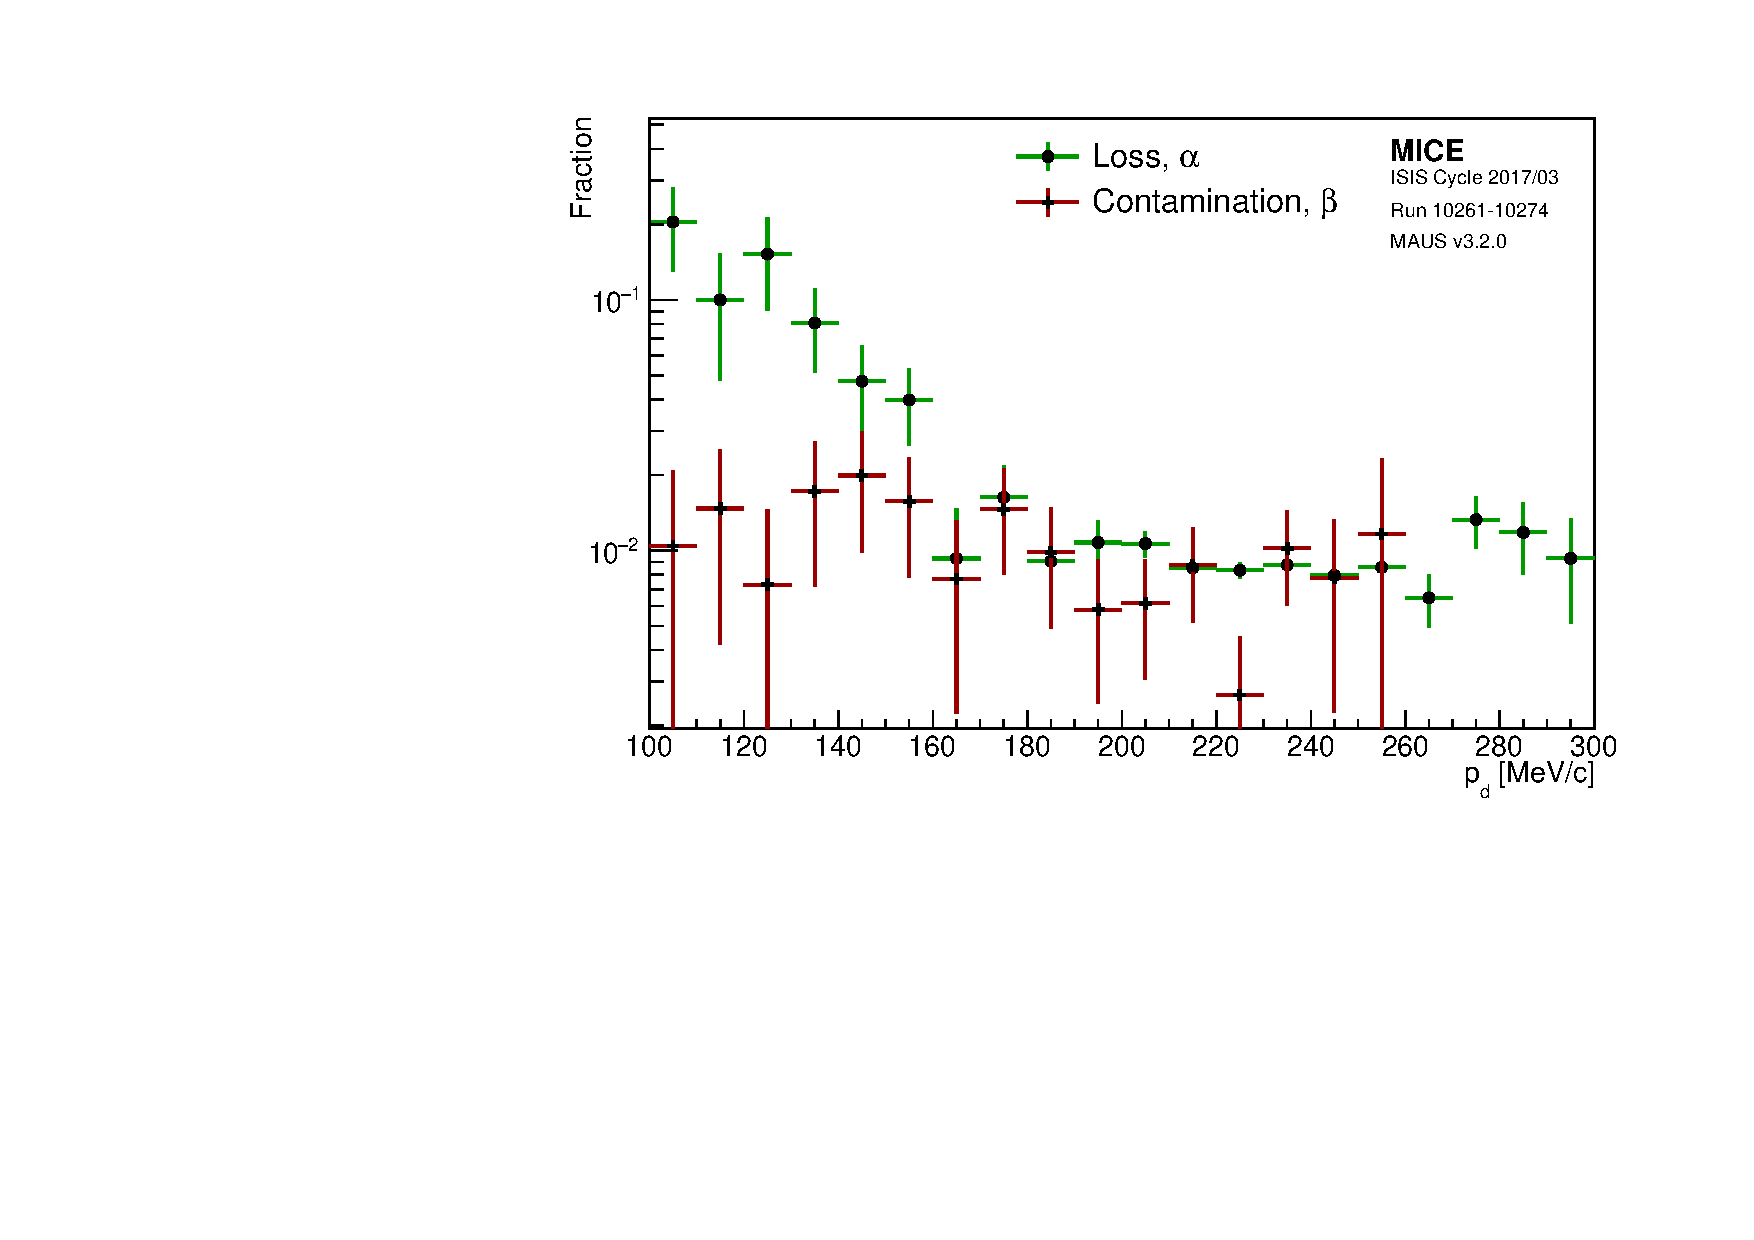
\includegraphics[width=0.68\columnwidth]{pid_mom.pdf}  		
		\caption{Percentage of electron contamination, $\beta$, and muon loss, $\alpha$, for different ranges of momentum measured in the downstream tracker, $p_d$. The error bars are based on the statistical uncertainty in a bin.}
		\label{fig:emr_pid_mom}
	\end{center}
\end{figure}
